% Options for packages loaded elsewhere
\PassOptionsToPackage{unicode}{hyperref}
\PassOptionsToPackage{hyphens}{url}
\documentclass[
  11pt,
]{article}
\usepackage{xcolor}
\usepackage[left=3cm,right=3cm,top=2.5cm,bottom=2.5cm]{geometry}
\usepackage{amsmath,amssymb}
\setcounter{secnumdepth}{5}
\usepackage{iftex}
\ifPDFTeX
  \usepackage[T1]{fontenc}
  \usepackage[utf8]{inputenc}
  \usepackage{textcomp} % provide euro and other symbols
\else % if luatex or xetex
  \usepackage{unicode-math} % this also loads fontspec
  \defaultfontfeatures{Scale=MatchLowercase}
  \defaultfontfeatures[\rmfamily]{Ligatures=TeX,Scale=1}
\fi
\usepackage{lmodern}
\ifPDFTeX\else
  % xetex/luatex font selection
\fi
% Use upquote if available, for straight quotes in verbatim environments
\IfFileExists{upquote.sty}{\usepackage{upquote}}{}
\IfFileExists{microtype.sty}{% use microtype if available
  \usepackage[]{microtype}
  \UseMicrotypeSet[protrusion]{basicmath} % disable protrusion for tt fonts
}{}
\usepackage{setspace}
\makeatletter
\@ifundefined{KOMAClassName}{% if non-KOMA class
  \IfFileExists{parskip.sty}{%
    \usepackage{parskip}
  }{% else
    \setlength{\parindent}{0pt}
    \setlength{\parskip}{6pt plus 2pt minus 1pt}}
}{% if KOMA class
  \KOMAoptions{parskip=half}}
\makeatother
\usepackage{longtable,booktabs,array}
\usepackage{caption}
\captionsetup[table]{skip=6pt}
\newcounter{none} % for unnumbered tables
\usepackage{calc} % for calculating minipage widths
% Correct order of tables after \paragraph or \subparagraph
\usepackage{etoolbox}
\makeatletter
\patchcmd\longtable{\par}{\if@noskipsec\mbox{}\fi\par}{}{}
\makeatother
% Allow footnotes in longtable head/foot
\IfFileExists{footnotehyper.sty}{\usepackage{footnotehyper}}{\usepackage{footnote}}
\makesavenoteenv{longtable}
\usepackage{graphicx}
\makeatletter
\newsavebox\pandoc@box
\newcommand*\pandocbounded[1]{% scales image to fit in text height/width
  \sbox\pandoc@box{#1}%
  \Gscale@div\@tempa{\textheight}{\dimexpr\ht\pandoc@box+\dp\pandoc@box\relax}%
  \Gscale@div\@tempb{\linewidth}{\wd\pandoc@box}%
  \ifdim\@tempb\p@<\@tempa\p@\let\@tempa\@tempb\fi% select the smaller of both
  \ifdim\@tempa\p@<\p@\scalebox{\@tempa}{\usebox\pandoc@box}%
  \else\usebox{\pandoc@box}%
  \fi%
}
% Set default figure placement to htbp
\def\fps@figure{htbp}
\makeatother
\setlength{\emergencystretch}{3em} % prevent overfull lines
\providecommand{\tightlist}{%
  \setlength{\itemsep}{0pt}\setlength{\parskip}{0pt}}
%% tools/stamp.tex
%% Provenance footer for PDFs rendered from this project.
%% Vendored by zzcollab; this file is not project-specific. The
%% footer prints the source document and the time of rendering.
%% The git version is defined here too, and so is available to a
%% project that wants it on the page, but it is left off the
%% default footer: it already names the staged copy in share/ and
%% appears in its manifest row. All values are supplied at render
%% time by tools/stamp-render.R, which writes a small generated
%% file that redefines the macros below. The \providecommand
%% defaults keep a bare LaTeX compile working when the document is
%% built without the wrapper.
\usepackage{fancyhdr}
\usepackage{xcolor}
\providecommand{\stampsource}{\detokenize{(source not recorded)}}
\providecommand{\stamptime}{(time not recorded)}
\providecommand{\stampversion}{\detokenize{(version not recorded)}}
\setlength{\footskip}{40pt}
\newcommand{\stampfootcontent}{%
  \footnotesize\color{gray}%
  \parbox[b]{\textwidth}{%
    \stamptime\hfill\thepage\\[2pt]%
    \ttfamily\raggedright\stampsource}}
\pagestyle{fancy}
\fancyhf{}
\fancyfoot[C]{\stampfootcontent}
\renewcommand{\headrulewidth}{0pt}
\renewcommand{\footrulewidth}{0.4pt}
%% The title page uses the `plain` page style; redefine it so the
%% stamp appears there too.
\fancypagestyle{plain}{%
  \fancyhf{}%
  \fancyfoot[C]{\stampfootcontent}%
  \renewcommand{\headrulewidth}{0pt}%
  \renewcommand{\footrulewidth}{0.4pt}}
\renewcommand{\stampsource}{\textasciitilde{}/\allowbreak{}prj/\allowbreak{}res/\allowbreak{}36-pmsimstats-ng/\allowbreak{}pmsimstats-ng/\allowbreak{}analysis/\allowbreak{}report/\allowbreak{}02-carryover-sensitivity/\allowbreak{}report-devresults.Rmd}
\renewcommand{\stamptime}{2026-08-15 16:48 PDT}
\renewcommand{\stampversion}{\detokenize{bc0b671-wip}}
\usepackage{amsmath}
\usepackage{amssymb}
\usepackage{booktabs}
\usepackage{longtable}
\usepackage{float}
\usepackage[mathlines]{lineno}
\linenumbers
\usepackage{bookmark}
\IfFileExists{xurl.sty}{\usepackage{xurl}}{} % add URL line breaks if available
\urlstyle{same}
% fallback for those not using the hyperref driver hyperxmp:
\makeatletter
\@ifundefined{xmpquote}{\newcommand{\xmpquote}[1]{#1}}{}
\makeatother
\hypersetup{
  pdftitle={Carryover-sensitivity study: development-run review},
  pdfauthor={pmsimstats team},
  hidelinks,
  pdfcreator={LaTeX via pandoc}}

\title{Carryover-sensitivity study: development-run review}
\usepackage{etoolbox}
\makeatletter
\providecommand{\subtitle}[1]{% add subtitle to \maketitle
  \apptocmd{\@title}{\par {\large #1 \par}}{}{}
}
\makeatother
\subtitle{96-cell grid, five analysis methods, 150 replicates per cell}
\author{pmsimstats team}
\date{August 15, 2026}

\begin{document}
\maketitle

{
\setcounter{tocdepth}{2}
\tableofcontents
}
\setstretch{1.1}
\section{Overview}\label{overview}

This document presents pipeline-verification results for the
carryover-sensitivity manuscript from the development simulation
run completed 2026-05-20. The run uses a 96-cell reduced Tier 1
grid (150 replicates per cell, MCSE \(\approx 0.041\) at \(p = 0.5\))
and a 31-cell Tier 2 sensitivity grid. All figures and tables are
computed inline from the development RDS files; nothing is loaded
from pre-rendered figures or the shared \texttt{analysis/data/} summaries.

\textbf{Five analysis methods.} Beyond the three analysis-model
specifications of the parent study, E1 (binary \(D_b\)), E2
(exposure-weighted \(D_{bc}\)), and E3 (lagged-treatment), this dev
run carries two robust-inference analyses, both applied to the E2
(\(D_{bc}\)) predictor. \texttt{lme+CR2} is the conditional \texttt{lme} fit with
its model-based standard error replaced by a CR2 bias-reduced
cluster-robust sandwich. \texttt{GEE+MD} is the marginal
generalized-estimating-equations fit with a Mancl-DeRouen
bias-corrected sandwich. The two robust analyses are produced by
the \texttt{-\/-robust} flag of the simulation drivers, in anticipation of
carrying them into the production pipeline; their rationale and
validation are documented in manuscript 10
(\texttt{analysis/report/10-interaction-test-calibration/}).

The purpose of this document is to verify that:

\begin{enumerate}
\def\labelenumi{\alph{enumi})}
\tightlist
\item
  the E2 \(>\) E1 \(\approx\) E3 power ranking is visible at 150 reps;
\item
  the three model-based specifications are conservative under the
  null, while the robust analyses move the Type I error toward
  the nominal 0.05;
\item
  lme+CR2 recovers the power lost to conservatism, while GEE+MD
  carries a modest residual efficiency cost as a marginal-model
  estimator;
\item
  the Tier 2 sensitivity-block trends are plausible.
\end{enumerate}

Precise point estimates should be drawn from the production run
(500 reps, 540 cells) rather than from this document.

\textbf{Dev grid coverage.} The Tier 1 dev grid retains both DGP
architectures and all three DGP decay forms (the primary axes),
trimming secondary axes to two representative values each.
\texttt{t1half} is reduced to \(\{0.0, 1.0\}\) weeks; design to
\(\{\text{CO}, \text{Hybrid}\}\); \(N\) to \(\{35, 70\}\); \(c_{bm}\) to
\(\{0.0, 0.45\}\); Weibull uses only \(k = 0.7\). The OL+BDC design and
\(k = 1.5\) Weibull shape are absent from the dev grid; any figure
filtered to those levels will appear empty.

\begin{table}

\caption{\label{tab:meta-table}Development-run metadata read from the output RDS files.}
\centering
\begin{tabular}[t]{ll}
\toprule
Item & Value\\
\midrule
Tier 1 cells & 96\\
Tier 1 reps/cell & 150\\
Tier 2 cells & 31\\
Tier 2 reps/cell & 150\\
Analysis methods per cell & 5\\
\addlinespace
Total Tier 1 rows & 72000\\
Total Tier 2 rows & 23250\\
Run date & 2026-05-21\\
\bottomrule
\end{tabular}
\end{table}

\section{Tier 1 results}\label{tier-1-results}

\subsection{Headline performance at the reference cell}\label{headline-performance-at-the-reference-cell}

Table \ref{tab:headline-dev} shows the Morris-style performance
measures at the reference cell (the covariance-moderation architecture, exponential DGP,
Hybrid design, \(N = 70\), \(c_{bm} = 0.45\)), for all five analysis
methods at both carryover half-lives present in the dev grid.

\begin{table}

\caption{\label{tab:headline-dev}Reference-cell performance (the covariance-moderation architecture, exponential
    DGP, Hybrid, $N = 70$, $c_{bm} = 0.45$, $n_{sim} = 150$). The
    lme+CR2 row shares the E2 interaction estimate (its bias and
    empirical SE track E2) and differs only in the standard error;
    GEE+MD is a separate marginal fit with its own estimate,
    modestly less efficient than the conditional lme. MCSEs are
    about twice those of the 500-rep production run.}
\centering
\begin{tabular}[t]{rllllll}
\toprule
t1/2 & spec & Power (MCSE) & Bias (MCSE) & Emp SE & Coverage & Non-conv\\
\midrule
0 & E1 & 0.967 (0.015) & +0.043 (0.071) & 0.870 & 0.953 & 0.000\\
0 & E2 & 0.967 (0.015) & +0.043 (0.071) & 0.870 & 0.953 & 0.000\\
0 & E3 & 0.967 (0.015) & +0.044 (0.071) & 0.866 & 0.953 & 0.000\\
0 & lme+CR2 & 0.987 (0.009) & +0.043 (0.071) & 0.873 & 0.906 & 0.007\\
0 & GEE+MD & 0.960 (0.016) & +0.095 (0.074) & 0.908 & 0.913 & 0.000\\
\addlinespace
1 & E1 & 0.727 (0.036) & +1.231 (0.065) & 0.792 & 0.767 & 0.000\\
1 & E2 & 0.873 (0.027) & +0.098 (0.081) & 0.997 & 1.000 & 0.000\\
1 & E3 & 0.720 (0.037) & +1.249 (0.066) & 0.804 & 0.767 & 0.000\\
1 & lme+CR2 & 0.893 (0.025) & +0.095 (0.082) & 0.999 & 0.946 & 0.007\\
1 & GEE+MD & 0.847 (0.029) & +0.068 (0.086) & 1.058 & 0.960 & 0.000\\
\bottomrule
\end{tabular}
\end{table}

\subsection{Power by analysis method}\label{power-by-analysis-method}

\begin{figure}
\centering
\pandocbounded{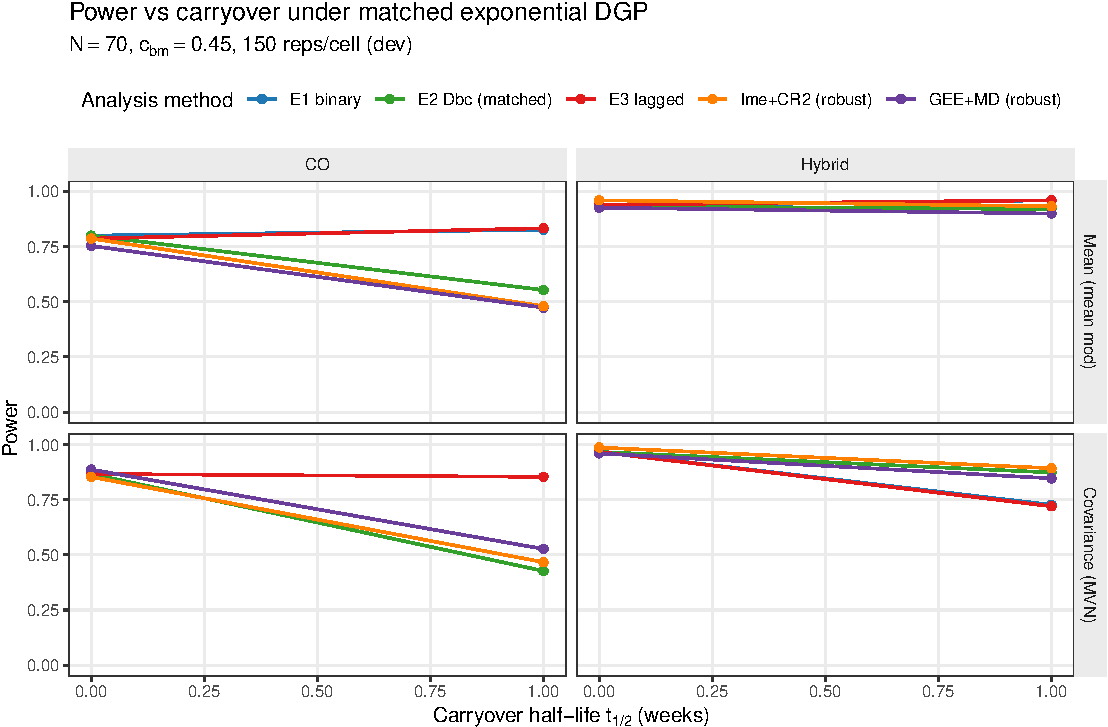
\includegraphics[keepaspectratio,alt={\label{fig:fig-power-by-spec}Power versus carryover half-life under the exponential DGP, stratified by architecture and design, for all five analysis methods. Dev grid: design in \{CO, Hybrid\} only; N = 70, c\_\{bm\} = 0.45, 150 reps per cell. lme+CR2 lifts power above E2 by recalibrating the conservative standard error; GEE+MD tracks just below E2, a modest residual efficiency cost of the marginal estimator relative to the conditional lme.}]{report-devresults_files/report-devresults_files/figure-latex/fig-power-by-spec-1.pdf}}
\caption{\label{fig:fig-power-by-spec}Power versus carryover half-life under the exponential DGP, stratified by architecture and design, for all five analysis methods. Dev grid: design in \{CO, Hybrid\} only; \(N = 70\), \(c_{bm} = 0.45\), 150 reps per cell. lme+CR2 lifts power above E2 by recalibrating the conservative standard error; GEE+MD tracks just below E2, a modest residual efficiency cost of the marginal estimator relative to the conditional lme.}
\end{figure}

\subsection{Decay-form by analysis-method heatmap}\label{decay-form-by-analysis-method-heatmap}

\begin{figure}
\centering
\pandocbounded{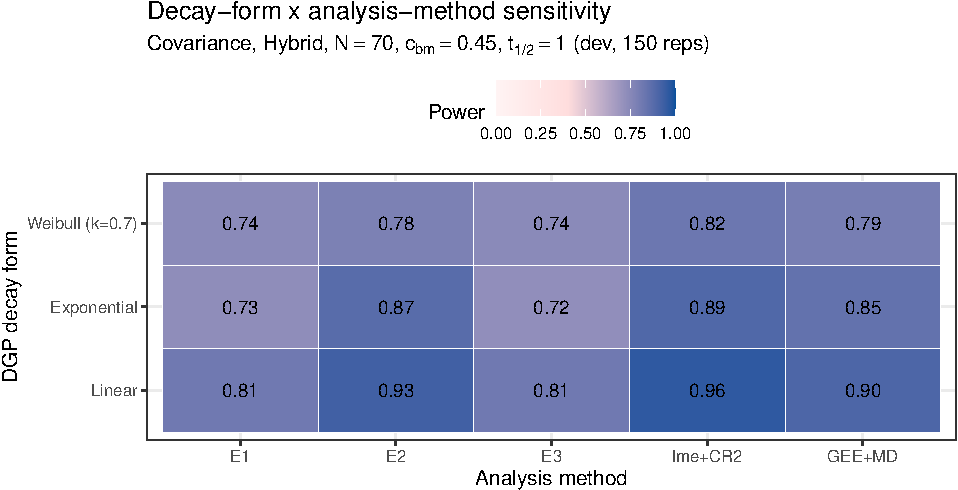
\includegraphics[keepaspectratio,alt={\label{fig:fig-heatmap}Power at the reference carryover cell (t\_\{1/2\} = 1.0 week, the covariance-moderation architecture, Hybrid design, N = 70, c\_\{bm\} = 0.45) across DGP decay forms and the five analysis methods. The dev grid contains three DGP forms: Linear, Exponential, and Weibull k = 0.7.}]{report-devresults_files/report-devresults_files/figure-latex/fig-heatmap-1.pdf}}
\caption{\label{fig:fig-heatmap}Power at the reference carryover cell (\(t_{1/2} = 1.0\) week, the covariance-moderation architecture, Hybrid design, \(N = 70\), \(c_{bm} = 0.45\)) across DGP decay forms and the five analysis methods. The dev grid contains three DGP forms: Linear, Exponential, and Weibull \(k = 0.7\).}
\end{figure}

\subsection{Type I error control}\label{type-i-error-control}

\begin{figure}
\centering
\pandocbounded{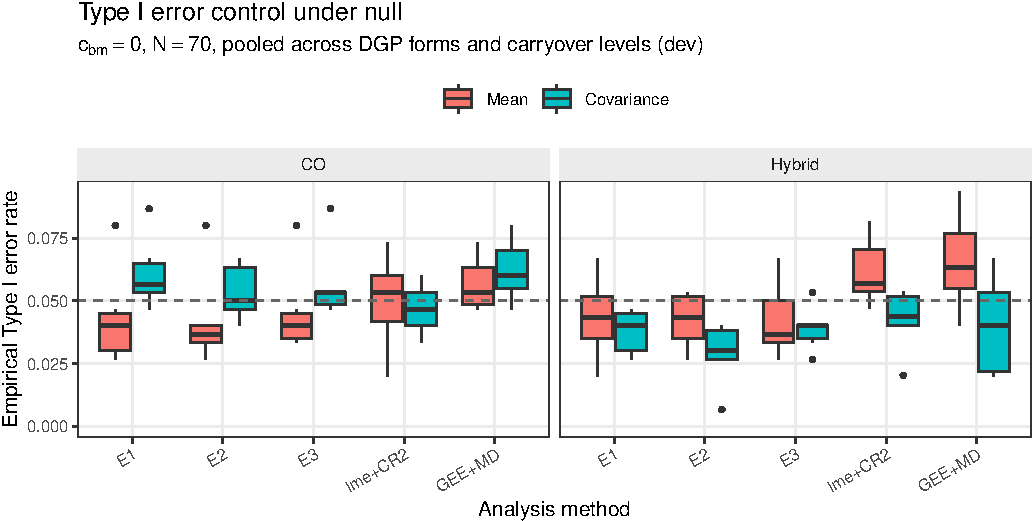
\includegraphics[keepaspectratio,alt={\label{fig:fig-type1}Empirical Type I error rates under the null (c\_\{bm\} = 0), pooled across DGP decay forms and carryover half-lives, stratified by design and analysis method. N = 70; dashed line at nominal 0.05. The three model-based specifications sit below nominal; lme+CR2 sits near nominal; GEE+MD is near nominal under the Hybrid design but anti-conservative under CO.}]{report-devresults_files/report-devresults_files/figure-latex/fig-type1-1.pdf}}
\caption{\label{fig:fig-type1}Empirical Type I error rates under the null (\(c_{bm} = 0\)), pooled across DGP decay forms and carryover half-lives, stratified by design and analysis method. \(N = 70\); dashed line at nominal 0.05. The three model-based specifications sit below nominal; lme+CR2 sits near nominal; GEE+MD is near nominal under the Hybrid design but anti-conservative under CO.}
\end{figure}

The three model-based specifications E1, E2, and E3 sit visibly
below the nominal 0.05 line in Figure \ref{fig:fig-type1}, the
conservatism diagnosed in manuscript 10
(\texttt{analysis/report/10-interaction-test-calibration/}); lme+CR2 and
GEE+MD sit on or near it, confirming that the robust analyses
recalibrate the interaction test. Figure
\ref{fig:fig-type1-arch} shows the same null cells split by DGP
architecture rather than by design. Because the two architectures
reduce to a bit-identical data-generating process when
\(c_{bm} = 0\), the Mean and Covariance panels are two samples from
one distribution and should coincide up to Monte Carlo noise; that
they do is a consistency check on the simulation.

\begin{figure}
\centering
\pandocbounded{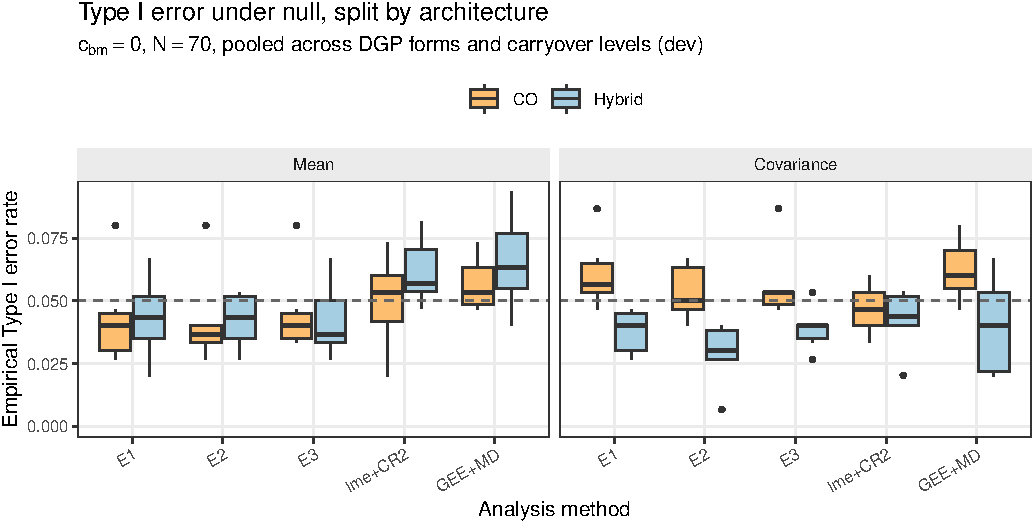
\includegraphics[keepaspectratio,alt={\label{fig:fig-type1-arch}Empirical Type I error rates under the null (c\_\{bm\} = 0, N = 70), the same null cells as the preceding figure but split by DGP architecture, with design as the fill. At the null the two architectures are a bit-identical data-generating process, so the two panels coincide up to Monte Carlo noise. Dashed line at nominal 0.05.}]{report-devresults_files/report-devresults_files/figure-latex/fig-type1-arch-1.pdf}}
\caption{\label{fig:fig-type1-arch}Empirical Type I error rates under the null (\(c_{bm} = 0\), \(N = 70\)), the same null cells as the preceding figure but split by DGP architecture, with design as the fill. At the null the two architectures are a bit-identical data-generating process, so the two panels coincide up to Monte Carlo noise. Dashed line at nominal 0.05.}
\end{figure}

\subsection{\texorpdfstring{Summary table: all cells at \(N = 70\), \(c_{bm} = 0.45\), Hybrid}{Summary table: all cells at N = 70, c\_\{bm\} = 0.45, Hybrid}}\label{summary-table-all-cells-at-n-70-c_bm-0.45-hybrid}

\begin{longtable}[t]{llrlll}
\caption{\label{tab:all-cells-table}Power and non-convergence at $N = 70$, $c_{bm} = 0.45$,
    Hybrid design, dev grid (150 reps per cell), for all five
    analysis methods across the DGP-architecture combinations
    present in the dev grid.}\\
\toprule
Arch & DGP & t1/2 & spec & Power (MCSE) & Non-conv\\
\midrule
A & exponential & 0 & E1 & 0.933 (0.020) & 0.000\\
A & exponential & 0 & E2 & 0.933 (0.020) & 0.000\\
A & exponential & 0 & E3 & 0.940 (0.019) & 0.000\\
A & exponential & 0 & lme+CR2 & 0.960 (0.016) & 0.000\\
A & exponential & 0 & GEE+MD & 0.927 (0.021) & 0.000\\
\addlinespace
A & exponential & 1 & E1 & 0.960 (0.016) & 0.000\\
A & exponential & 1 & E2 & 0.920 (0.022) & 0.000\\
A & exponential & 1 & E3 & 0.960 (0.016) & 0.000\\
A & exponential & 1 & lme+CR2 & 0.933 (0.020) & 0.007\\
A & exponential & 1 & GEE+MD & 0.900 (0.024) & 0.000\\
\addlinespace
A & linear & 0 & E1 & 0.967 (0.015) & 0.000\\
A & linear & 0 & E2 & 0.967 (0.015) & 0.000\\
A & linear & 0 & E3 & 0.967 (0.015) & 0.000\\
A & linear & 0 & lme+CR2 & 0.966 (0.015) & 0.007\\
A & linear & 0 & GEE+MD & 0.947 (0.018) & 0.000\\
\addlinespace
A & linear & 1 & E1 & 0.967 (0.015) & 0.000\\
A & linear & 1 & E2 & 0.867 (0.028) & 0.000\\
A & linear & 1 & E3 & 0.960 (0.016) & 0.000\\
A & linear & 1 & lme+CR2 & 0.886 (0.026) & 0.007\\
A & linear & 1 & GEE+MD & 0.880 (0.027) & 0.000\\
\addlinespace
A & weibull k=0.7 & 0 & E1 & 0.993 (0.007) & 0.000\\
A & weibull k=0.7 & 0 & E2 & 0.993 (0.007) & 0.000\\
A & weibull k=0.7 & 0 & E3 & 1.000 (0.000) & 0.000\\
A & weibull k=0.7 & 0 & lme+CR2 & 0.993 (0.007) & 0.007\\
A & weibull k=0.7 & 0 & GEE+MD & 0.960 (0.016) & 0.000\\
\addlinespace
A & weibull k=0.7 & 1 & E1 & 0.973 (0.013) & 0.000\\
A & weibull k=0.7 & 1 & E2 & 0.947 (0.018) & 0.000\\
A & weibull k=0.7 & 1 & E3 & 0.973 (0.013) & 0.000\\
A & weibull k=0.7 & 1 & lme+CR2 & 0.973 (0.013) & 0.000\\
A & weibull k=0.7 & 1 & GEE+MD & 0.927 (0.021) & 0.000\\
\addlinespace
B & exponential & 0 & E1 & 0.967 (0.015) & 0.000\\
B & exponential & 0 & E2 & 0.967 (0.015) & 0.000\\
B & exponential & 0 & E3 & 0.967 (0.015) & 0.000\\
B & exponential & 0 & lme+CR2 & 0.987 (0.009) & 0.007\\
B & exponential & 0 & GEE+MD & 0.960 (0.016) & 0.000\\
\addlinespace
B & exponential & 1 & E1 & 0.727 (0.036) & 0.000\\
B & exponential & 1 & E2 & 0.873 (0.027) & 0.000\\
B & exponential & 1 & E3 & 0.720 (0.037) & 0.000\\
B & exponential & 1 & lme+CR2 & 0.893 (0.025) & 0.007\\
B & exponential & 1 & GEE+MD & 0.847 (0.029) & 0.000\\
\addlinespace
B & linear & 0 & E1 & 0.980 (0.011) & 0.000\\
B & linear & 0 & E2 & 0.980 (0.011) & 0.000\\
B & linear & 0 & E3 & 0.980 (0.011) & 0.000\\
B & linear & 0 & lme+CR2 & 0.980 (0.012) & 0.013\\
B & linear & 0 & GEE+MD & 0.953 (0.017) & 0.000\\
\addlinespace
B & linear & 1 & E1 & 0.813 (0.032) & 0.000\\
B & linear & 1 & E2 & 0.927 (0.021) & 0.000\\
B & linear & 1 & E3 & 0.813 (0.032) & 0.000\\
B & linear & 1 & lme+CR2 & 0.959 (0.016) & 0.013\\
B & linear & 1 & GEE+MD & 0.900 (0.024) & 0.000\\
\addlinespace
B & weibull k=0.7 & 0 & E1 & 1.000 (0.000) & 0.000\\
B & weibull k=0.7 & 0 & E2 & 1.000 (0.000) & 0.000\\
B & weibull k=0.7 & 0 & E3 & 1.000 (0.000) & 0.000\\
B & weibull k=0.7 & 0 & lme+CR2 & 1.000 (0.000) & 0.020\\
B & weibull k=0.7 & 0 & GEE+MD & 0.987 (0.009) & 0.000\\
\addlinespace
B & weibull k=0.7 & 1 & E1 & 0.740 (0.036) & 0.000\\
B & weibull k=0.7 & 1 & E2 & 0.780 (0.034) & 0.000\\
B & weibull k=0.7 & 1 & E3 & 0.740 (0.036) & 0.000\\
B & weibull k=0.7 & 1 & lme+CR2 & 0.824 (0.031) & 0.013\\
B & weibull k=0.7 & 1 & GEE+MD & 0.793 (0.033) & 0.000\\
\bottomrule
\end{longtable}

\section{Tier 2 sensitivity results}\label{tier-2-sensitivity-results}

\subsection{S1: within-factor autocorrelation}\label{s1-within-factor-autocorrelation}

\begin{figure}
\centering
\pandocbounded{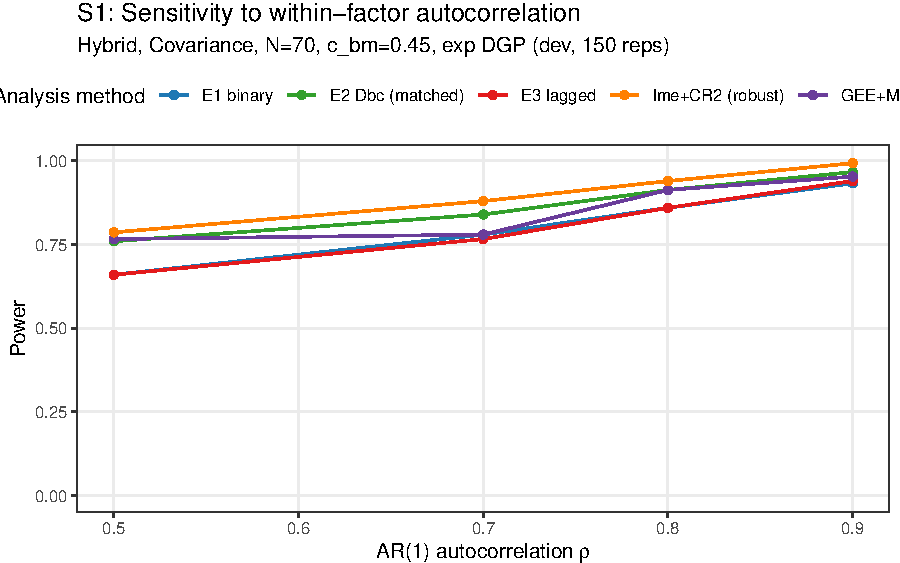
\includegraphics[keepaspectratio,alt={\label{fig:fig-s1}Power by analysis method across AR(1) autocorrelation \textbackslash rho \textbackslash in \textbackslash\{0.5, 0.7, 0.8, 0.9\textbackslash\}. Reference: Covariance, Hybrid, N = 70, c\_\{bm\} = 0.45, exponential DGP, t\_\{1/2\} = 1.0 weeks.}]{report-devresults_files/report-devresults_files/figure-latex/fig-s1-1.pdf}}
\caption{\label{fig:fig-s1}Power by analysis method across AR(1) autocorrelation \(\rho \in \{0.5, 0.7, 0.8, 0.9\}\). Reference: Covariance, Hybrid, \(N = 70\), \(c_{bm} = 0.45\), exponential DGP, \(t_{1/2} = 1.0\) weeks.}
\end{figure}

\subsection{S2: analyst-truth half-life mismatch}\label{s2-analyst-truth-half-life-mismatch}

\begin{figure}
\centering
\pandocbounded{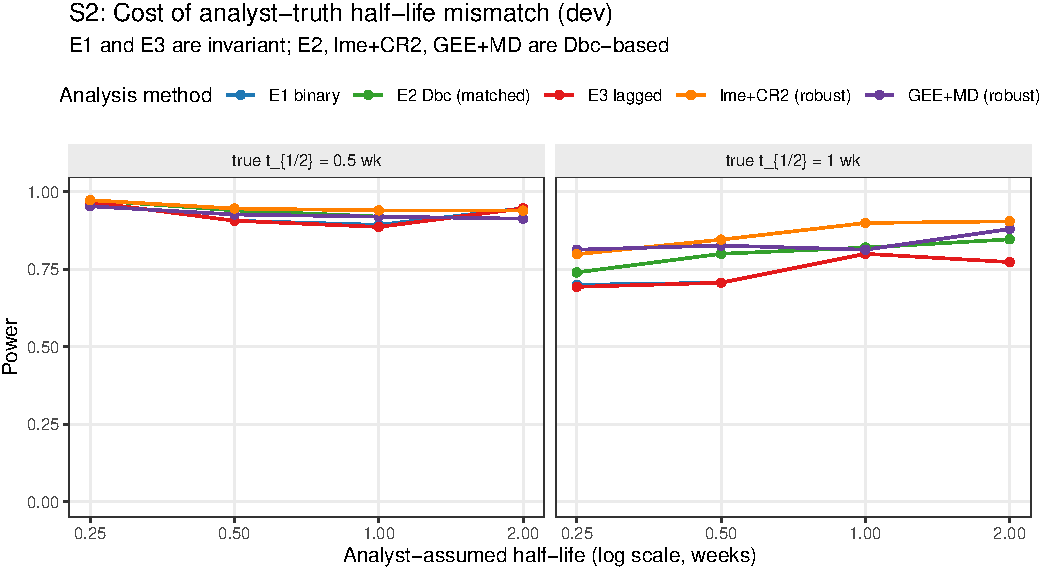
\includegraphics[keepaspectratio,alt={\label{fig:fig-s2}Power as the analyst's assumed half-life departs from the true DGP half-life. E1 and E3 do not consume the assumed half-life and are flat; E2 and the two robust analyses are all built on the D\_\{bc\} predictor and vary with it.}]{report-devresults_files/report-devresults_files/figure-latex/fig-s2-1.pdf}}
\caption{\label{fig:fig-s2}Power as the analyst's assumed half-life departs from the true DGP half-life. E1 and E3 do not consume the assumed half-life and are flat; E2 and the two robust analyses are all built on the \(D_{bc}\) predictor and vary with it.}
\end{figure}

\subsection{S3: dropout}\label{s3-dropout}

\begin{figure}
\centering
\pandocbounded{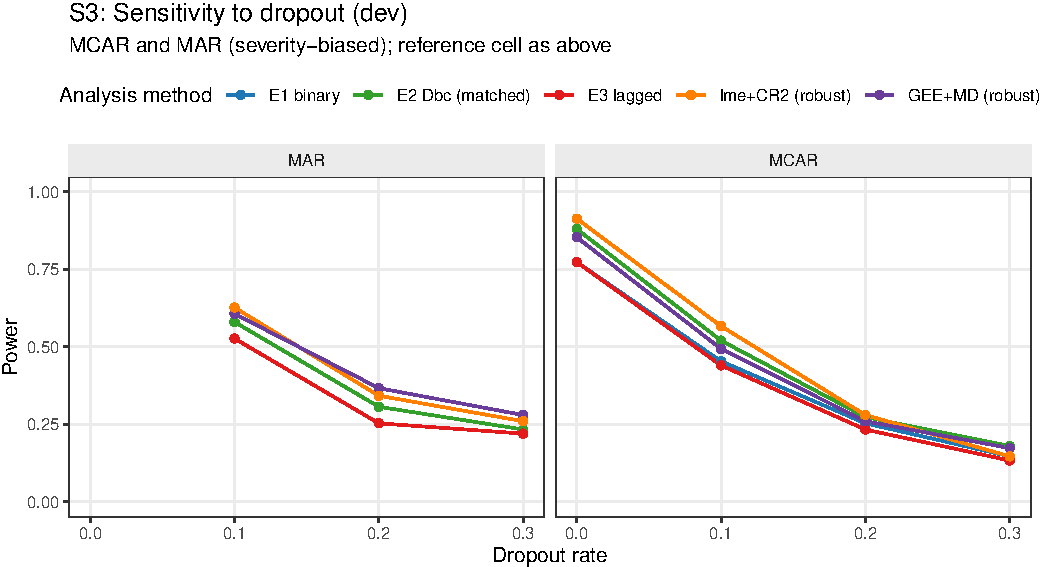
\includegraphics[keepaspectratio,alt={\label{fig:fig-s3}Power at dropout rates \textbackslash in \textbackslash\{0, 0.1, 0.2, 0.3\textbackslash\} under MCAR and MAR mechanisms, for all five analysis methods. With its exchangeable working correlation GEE+MD runs cleanly across the dropout range, power declining monotonically as expected.}]{report-devresults_files/report-devresults_files/figure-latex/fig-s3-1.pdf}}
\caption{\label{fig:fig-s3}Power at dropout rates \(\in \{0, 0.1, 0.2, 0.3\}\) under MCAR and MAR mechanisms, for all five analysis methods. With its exchangeable working correlation GEE+MD runs cleanly across the dropout range, power declining monotonically as expected.}
\end{figure}

\subsection{S4: biomarker-moderation effect-size curve}\label{s4-biomarker-moderation-effect-size-curve}

\begin{figure}
\centering
\pandocbounded{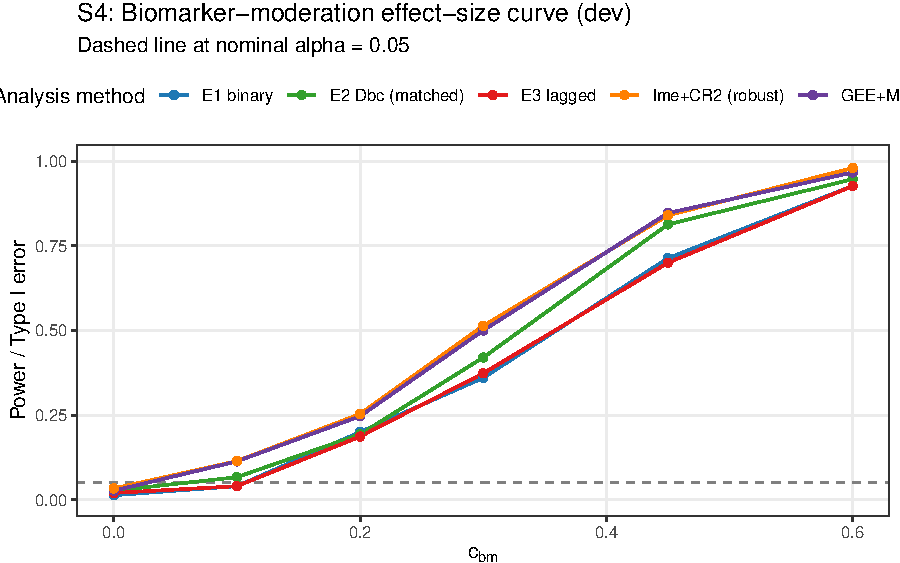
\includegraphics[keepaspectratio,alt={\label{fig:fig-s4}Power across c\_\{bm\} \textbackslash in \textbackslash\{0, 0.10, 0.20, 0.30, 0.45, 0.60\textbackslash\}, for all five analysis methods. The c\_\{bm\} = 0 point is the null; dashed line at nominal \textbackslash alpha = 0.05.}]{report-devresults_files/report-devresults_files/figure-latex/fig-s4-1.pdf}}
\caption{\label{fig:fig-s4}Power across \(c_{bm} \in \{0, 0.10, 0.20, 0.30, 0.45, 0.60\}\), for all five analysis methods. The \(c_{bm} = 0\) point is the null; dashed line at nominal \(\alpha = 0.05\).}
\end{figure}

\subsection{S5: autocorrelation by carryover (exploratory)}\label{s5-autocorrelation-by-carryover-exploratory}

\begin{figure}
\centering
\pandocbounded{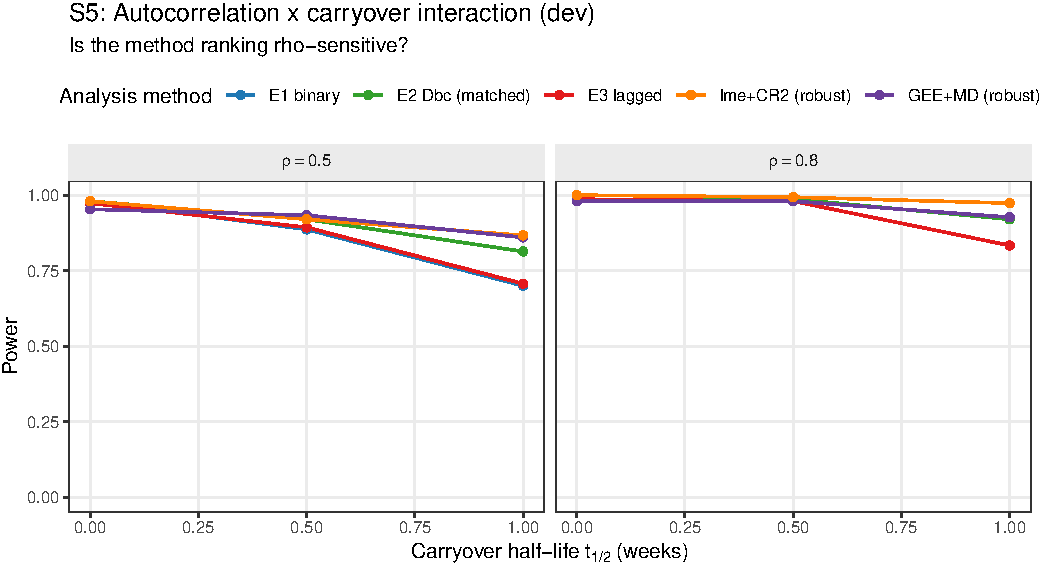
\includegraphics[keepaspectratio,alt={\label{fig:fig-s5}Power across carryover half-lives \textbackslash\{0, 0.5, 1.0\textbackslash\} weeks at \textbackslash rho \textbackslash in \textbackslash\{0.5, 0.8\textbackslash\}, for all five analysis methods. Facets by \textbackslash rho.}]{report-devresults_files/report-devresults_files/figure-latex/fig-s5-1.pdf}}
\caption{\label{fig:fig-s5}Power across carryover half-lives \(\{0, 0.5, 1.0\}\) weeks at \(\rho \in \{0.5, 0.8\}\), for all five analysis methods. Facets by \(\rho\).}
\end{figure}

\section{Dev-run review checklist}\label{dev-run-review-checklist}

\begin{table}

\caption{\label{tab:checklist}Automated sanity checks against the dev-run results.
    Thresholds are deliberately loose (MCSE ~0.041 at 150 reps).}
\centering
\begin{tabular}[t]{ll}
\toprule
Check & Result\\
\midrule
E2 power > E1 power at the reference cell & E2=0.873, E1=0.727 -> PASS\\
lme+CR2 power >= E2 power (robust SE recovers power) & lme+CR2=0.893, E2=0.873 -> PASS\\
lme+CR2 null Type I within 0.015 of nominal 0.05 & lme+CR2 mean Type I=0.050 -> PASS\\
Max non-convergence rate below 0.20 & Max=0.020 -> PASS\\
\bottomrule
\end{tabular}
\end{table}

\begin{center}\rule{0.5\linewidth}{0.5pt}\end{center}

\emph{Dev review document rendered from
\texttt{analysis/report/02-carryover-sensitivity/report-devresults.Rmd}
on 2026-08-15 at 16:48 PDT.}
\emph{Source data: \texttt{output/01-dev.rds} (72000 rows),
\texttt{output/04-sensitivity-dev.rds} (23250 rows).}

\end{document}
